% homework/hw06x/hw06x.tex
% Year 7 - Extra Homework: one letter at a time.
%
% Goes out alongside Homework 6. Same framing rule as hw03x, hw04x and hw05x:
% nothing on the sheet says easy, basic, extra help, catch-up or revision, and
% no question is marked as being for anybody in particular. The cover states a
% fact, and it is a true one -- there is almost no arithmetic in Unit 2. Every
% number in it is small. What decides the answer is one letter and where you
% put it.
%
% THE SCAFFOLDING IS BORROWED FROM THE WORKBOOK'S OWN FOCUS PAGES, deliberately.
% Section 2.1's Focus exercise does five things this sheet does too:
%
%   * a picture of a bag you can see into, twice, then one you cannot (E1);
%   * a part-written sentence with a box to fill, walked from a known number to
%     an unknown one (E2);
%   * "the first one has been done for you" on every matching and true/false
%     question (E5, E6, E7, E9, E11, E12);
%   * one letter, one situation, four operations in a row (E4);
%   * a margin Tip that prints the middle line itself -- n - 1 = 5 - 1 = [] --
%     which is E8's whole design.
%
% E8 is the sheet in miniature. The middle line is printed as a skeleton with
% the numbers missing, so a student cannot skip it: filling the gaps IS the
% method. That is the one habit that fixes 3n = 34.
%
% Part 3 is the Section C bridge from Homework 6, taken slowly: cm, cm^2, cm^3
% as one length, two multiplied, three multiplied, and a tank whose base area
% is worked out before the letter ever appears.
%
% House style is shared: see homework/hw-style.tex. Method: the new-homework
% skill. Source is pure ASCII on purpose.
%
% Build:  pwsh .claude/skills/new-homework/scripts/build-hw.ps1 hw06x

\documentclass[12pt,a4paper]{article}

% -- Answer key switch -------------------------------------------------------
\newif\ifkey
\ifdefined\TEACHER\keytrue\else
  \keyfalse        % \keyfalse = student copy   |   \keytrue = teacher copy
\fi

% -- House style -------------------------------------------------------------
% homework/hw-style.tex
% Shared house style for every Year 7 homework packet. \input this from the
% packet file, right after \documentclass and the answer-key switch.
%
% Do not fork this file per packet. If a packet needs a different look, the
% question is whether every packet should have it.
%
% The choices here are deliberate and were arrived at by printing and looking:
%   * No solid dark banners. Every header is a light tint with a coloured spine
%     on the left, so colour reads clearly without flooding a school printer.
%   * No marks and no mark totals. These are practice, not exam papers.
%   * Lato at 12pt with open leading, plus mathastext so inline maths is Lato
%     too. Without mathastext every "-6 + 4" is Computer Modern serif and the
%     sheet looks half-typeset.
%   * Writing lines are spaced for Year 7 handwriting, not adult margin notes.
%
% Provides: \wlines \blank \tickbox \sep \qmk-free marks (none) \hwsection
% \qhead \expr, the workspace box, and the remember / wordhelp / activity /
% yourturn coloured boxes. Palette matches the lesson decks exactly.

% -- Packages ----------------------------------------------------------------
\usepackage[T1]{fontenc}
\usepackage[utf8]{inputenc}
\usepackage[default]{lato}
\usepackage[a4paper,top=1.7cm,bottom=1.7cm,left=2.0cm,right=2.0cm,headheight=15pt]{geometry}
\usepackage{amsmath,amssymb}
\usepackage{xcolor}
\usepackage[most]{tcolorbox}
\usepackage{enumitem}
\usepackage{tikz}
\usetikzlibrary{arrows.meta}
\usepackage{array}
\usepackage{tabularx}
\usepackage{fancyhdr}
\usepackage{multicol}
\usepackage{needspace}
\usepackage{graphicx}

% Make maths use Lato too. Without this, every "-6 + 4" on the page is set in
% Computer Modern serif and the sheet looks half-typeset. Must come last.
\usepackage[italic]{mathastext}

\linespread{1.06}\selectfont

% -- The Learner's Book palette (same hex values as the lesson decks) ---------
\definecolor{cbteal}{HTML}{0087A8}
\definecolor{cbpurple}{HTML}{5C2483}
\definecolor{cborange}{HTML}{C25E12}
\definecolor{cbgreen}{HTML}{4A8B23}
\definecolor{cbred}{HTML}{C8102E}
\definecolor{cbblue}{HTML}{1A5FA8}
\definecolor{rulegray}{HTML}{9AA5AD}

% -- Answer lines and blanks -------------------------------------------------
% \wlines{n} draws n ruled writing lines, spaced wide enough for Year 7
% handwriting rather than for an adult with a fine pen.
\makeatletter
\newcommand{\wlines}[1]{%
  \par\vspace{0.75em}%
  \@tempcnta=0\relax
  \@whilenum\@tempcnta<#1\do{%
    \hbox to \linewidth{\color{rulegray}\leaders\hrule height 0.5pt\hfill}%
    \vspace{1.5em}%
    \advance\@tempcnta by 1\relax}%
  \par\vspace{-0.8em}%
}
\makeatother

% \blank[width] is an inline gap to write a short answer in.
\newcommand{\blank}[1][2.6cm]{\underline{\hspace{#1}}}

% A boxed space for showing working.
\newtcolorbox{workspace}[1][3.4cm]{%
  colback=white, colframe=rulegray, boxrule=0.5pt, arc=5pt,
  height=#1, left=6pt, right=6pt, top=4pt, bottom=4pt,
  before skip=9pt, after skip=11pt}

% An empty tick box.
\newcommand{\tickbox}{\fbox{\rule{0pt}{1.15em}\rule{1.15em}{0pt}}}

% A middot separator.
\newcommand{\sep}{\,\textperiodcentered\,}

% -- Section and question headings -------------------------------------------
% Light tint plus a fat coloured spine on the left. No solid dark banner: the
% colour reads clearly but barely costs the printer anything.
% needspace stops a heading stranding alone at the foot of a page. Kept modest:
% too large and it pushes headings over, leaving a worse hole than it prevents.
\newcommand{\hwsection}[2][cbteal]{%
  \needspace{8\baselineskip}%
  \par\vspace{13pt}%
  \noindent
  \begin{tcolorbox}[enhanced, nobeforeafter, width=\textwidth,
      colback=#1!7, colframe=#1!7, arc=5pt,
      borderline west={5pt}{0pt}{#1},
      left=14pt, right=10pt, top=7pt, bottom=7pt]
    {\large\bfseries\color{#1}#2}
  \end{tcolorbox}%
  \par\vspace{9pt}}

% \qhead[colour]{A2}{Moving along the line} -- a question heading.
\newcommand{\qhead}[3][cbteal]{%
  \needspace{6\baselineskip}%
  \par\vspace{11pt}%
  \noindent{\large\bfseries\color{#1}#2}\quad{\large\bfseries #3}\par\vspace{4pt}}

% -- Coloured boxes ----------------------------------------------------------
% Shared look: rounded, light fill, coloured rule, coloured title text on a
% pale title strip rather than a dark one.
\tcbset{hwbox/.style={
  enhanced, breakable, arc=6pt, boxrule=1pt,
  left=11pt, right=11pt, top=8pt, bottom=8pt,
  fonttitle=\bfseries, attach boxed title to top left={xshift=12pt, yshift=-8pt},
  boxed title style={arc=4pt, boxrule=1pt, left=7pt, right=7pt, top=2pt, bottom=2pt},
  top=13pt}}

% Orange: things to remember. Matches the deck's "Write This Down".
\newtcolorbox{remember}[1][Remember from the lesson]{hwbox,
  colback=cborange!6, colframe=cborange, coltitle=cborange,
  colbacktitle=white, title={#1}}

% Blue: English help. The barrier in this class is the wording, not the maths.
\newtcolorbox{wordhelp}[1][Word help]{hwbox,
  colback=cbblue!6, colframe=cbblue, coltitle=cbblue,
  colbacktitle=white, title={#1}}

% Purple: an activity or instruction.
\newtcolorbox{activity}[1][How to do this homework]{hwbox,
  colback=cbpurple!6, colframe=cbpurple, coltitle=cbpurple,
  colbacktitle=white, title={#1}}

% Green: your turn / a friendly nudge.
\newtcolorbox{yourturn}[1][Your turn]{hwbox,
  colback=cbgreen!7, colframe=cbgreen, coltitle=cbgreen!75!black,
  colbacktitle=white, title={#1}}

% -- Shorthands --------------------------------------------------------------
\newcommand{\dC}{\,^{\circ}\mathrm{C}}          % use inside maths: $-8\dC$
\newcommand{\key}[1]{{\color{cborange}\textbf{#1}}}
\newcommand{\eng}[1]{{\color{cbblue}\textbf{#1}}}

\setlist[enumerate]{itemsep=8pt, topsep=5pt, leftmargin=*}
\setlist[itemize]{itemsep=4pt, topsep=4pt, leftmargin=*}
\renewcommand{\arraystretch}{1.45}

% -- An expression the student is asked to work from -------------------------
\newcommand{\expr}[1]{%
  \tcbox[on line, colback=cbgreen!10, colframe=cbgreen!55, boxrule=1pt, arc=4pt,
         left=9pt, right=9pt, top=4pt, bottom=4pt]{\large\bfseries $#1$}}

% -- Running head and foot ---------------------------------------------------
% The packet overrides \fancyhead[L] with its own title.
\pagestyle{fancy}
\fancyhf{}
\fancyhead[L]{\small\color{black!55}Year 7\sep Homework}
\fancyhead[R]{\small\color{black!55}Name: \blank[3.4cm]}
\fancyfoot[C]{\small\color{black!55}Page \thepage}
\renewcommand{\headrulewidth}{0pt}
\renewcommand{\headrule}{\vspace{2pt}\hbox to\headwidth{\color{cbteal!45}\leaders\hrule height 1.2pt\hfill}}



% -- Per-packet running head -------------------------------------------------
\fancyhead[L]{\small\color{black!55}Year 7\sep Extra Homework}

% -- A group of writing lines that will not be split -------------------------
% See the note in hw06.tex: \wlines is a run of separate boxes and TeX will
% break in the middle of one, stranding a single rule at the top of a page.
\newcommand{\qlines}[1]{\par\needspace{\numexpr#1+1\relax\baselineskip}\wlines{#1}}

% -- A box to write one number in --------------------------------------------
% The workbook's own scaffold: a part-written line with an empty square where
% the number goes. Filling the squares IS the method being taught, so it has to
% look like something you write in, not like a blank.
\newcommand{\nbox}{\ \fbox{\rule{0pt}{1.05em}\rule{1.0em}{0pt}}\ }

\begin{document}

% ===========================================================================
% COVER BLOCK
% ===========================================================================
\thispagestyle{fancy}

\begin{tcolorbox}[enhanced, colback=cbgreen!8, colframe=cbgreen!8, arc=7pt,
                  borderline west={6pt}{0pt}{cbgreen},
                  left=18pt, right=14pt, top=11pt, bottom=11pt]
  {\color{cbgreen!75!black}\bfseries YEAR 7\sep UNIT 2\sep EXTRA HOMEWORK}\\[6pt]
  {\color{cbgreen!70!black}\Huge\bfseries One Letter at a Time}\\[10pt]
  {\color{black!70}Expressions, substituting\sep and where volume comes from}
\end{tcolorbox}

\vspace{6pt}
\noindent
\begin{tabularx}{\textwidth}{@{}X X@{}}
  \textbf{Name:} \blank[5.6cm] & \textbf{Class:} \blank[5.6cm] \\
  \textbf{Date given:} \blank[4.6cm] &
  \textbf{Date due:} {\color{cbred}\bfseries Monday 14 September 2026} \\
\end{tabularx}

\vspace{4pt}
\begin{activity}[Why this sheet exists]
  There is almost \key{no arithmetic} in Unit 2. Every number in it is small.
  What decides the answer is \key{one letter} --- what it stands for, and where
  you put it.

  \medskip
  So this sheet does one letter at a time, and it shows you the
  \key{middle line} of every calculation with the numbers left out. Filling in
  those boxes is not extra working. It \key{is} the method.

  \medskip
  \eng{No calculator.} Write in every box.
\end{activity}

% ===========================================================================
% PART 1 -- WHAT A LETTER IS
% ===========================================================================
\hwsection[cbgreen]{Part 1 \textperiodcentered\ What a letter is}

\qhead[cbgreen]{E1}{The bag you cannot see into}

\noindent Write the number of counters in each bag. For the last one you cannot
count them, so \textbf{choose your own letter} instead.

\vspace{8pt}
\begin{center}
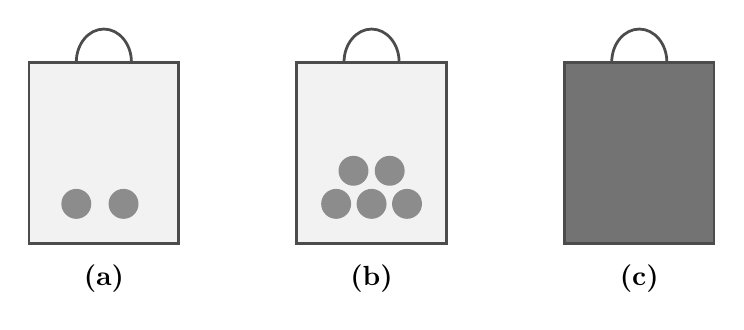
\begin{tikzpicture}[x=1cm, y=1cm, line width=1.0pt]

  % -- bag A: two counters, visible ---------------------------------------
  \begin{scope}[shift={(0,0)}]
    \fill[black!5] (0,0) rectangle (1.9,2.3);
    \draw[black!70] (0,0) rectangle (1.9,2.3);
    \draw[black!70] (0.6,2.3) arc (180:0:0.35 and 0.42);
    \fill[black!45] (0.6,0.5) circle (0.19);
    \fill[black!45] (1.2,0.5) circle (0.19);
  \end{scope}

  % -- bag B: five counters, visible --------------------------------------
  \begin{scope}[shift={(3.4,0)}]
    \fill[black!5] (0,0) rectangle (1.9,2.3);
    \draw[black!70] (0,0) rectangle (1.9,2.3);
    \draw[black!70] (0.6,2.3) arc (180:0:0.35 and 0.42);
    \fill[black!45] (0.5,0.5) circle (0.19);
    \fill[black!45] (0.95,0.5) circle (0.19);
    \fill[black!45] (1.4,0.5) circle (0.19);
    \fill[black!45] (0.72,0.92) circle (0.19);
    \fill[black!45] (1.18,0.92) circle (0.19);
  \end{scope}

  % -- bag C: solid, nothing visible. This is the whole idea of a letter. --
  \begin{scope}[shift={(6.8,0)}]
    \fill[black!55] (0,0) rectangle (1.9,2.3);
    \draw[black!70] (0,0) rectangle (1.9,2.3);
    \draw[black!70] (0.6,2.3) arc (180:0:0.35 and 0.42);
  \end{scope}

  \node[font=\bfseries] at (0.95,-0.45) {(a)};
  \node[font=\bfseries] at (4.35,-0.45) {(b)};
  \node[font=\bfseries] at (7.75,-0.45) {(c)};

\end{tikzpicture}
\end{center}

\vspace{6pt}
\noindent
\begin{tabular}{@{}p{0.31\textwidth} p{0.31\textwidth} p{0.31\textwidth}@{}}
  (a) \nbox counters &
  (b) \nbox counters &
  (c) \nbox counters \\
\end{tabular}

\begin{wordhelp}[Why (c) needs a letter]
  You cannot see inside bag (c), so nobody knows the number. That does not mean
  there is no number --- there is one, and you just cannot count it. So we give
  it a \eng{letter} instead, and carry on.
\end{wordhelp}

% -- E2 ---------------------------------------------------------------------
\qhead[cbgreen]{E2}{Put three more in}

\noindent Three counters are put into each bag. Fill in the boxes.

\vspace{4pt}
\begin{enumerate}[label=(\alph*), itemsep=13pt]
  \item There are \textbf{6} counters in the bag.

        Put in three more, so now there are \; $6 + 3 = \nbox$ \; counters.

  \item There are \textbf{10} counters in the bag.

        Put in three more, so now there are \; $\nbox + 3 = \nbox$ \; counters.

  \item There are \textbf{$n$} counters in the bag.

        Put in three more, so now there are \; $\nbox + 3$ \; counters.

  \item There are \textbf{$n$} counters in the bag.

        Take four out, so now there are \; $\nbox - \nbox$ \; counters.
\end{enumerate}

\begin{remember}[Part (c) is the one that matters]
  You \key{cannot} work out $n + 3$. There is nothing to work out --- you do not
  know what $n$ is. So you \key{leave it as it is}. $n + 3$ is the
  \key{finished answer}, and this is called an \key{expression}.
\end{remember}

% -- E3 ---------------------------------------------------------------------
\qhead[cbgreen]{E3}{Say it the short way}

\begin{remember}[The three rules]
  $4 \times n$ is written \key{4n} --- the number goes \key{in front}. \\
  $a \times b$ is written \key{ab}. \\
  $w \div 2$ is written \key{w over 2}, as a fraction.
\end{remember}

\noindent The first one is done for you.

\vspace{6pt}
\begin{multicols}{2}
\begin{enumerate}[label=(\alph*), itemsep=12pt]
  \item $4 \times n \;=\; \mathbf{4n}$
  \item $7 \times k \;=\;$ \blank[2.0cm]
  \item $m \times p \;=\;$ \blank[2.0cm]
  \item $3 \times a \times b \;=\;$ \blank[2.0cm]
  \item $w \div 2 \;=\;$ \blank[2.0cm]
  \item $t \div 5 \;=\;$ \blank[2.0cm]
\end{enumerate}
\end{multicols}

% -- E4 ---------------------------------------------------------------------
\qhead[cbgreen]{E4}{One beaker, four things to do to it}

\noindent Mr Bowen has a beaker holding \textbf{$b$ cm$^3$} of water. Nobody has
measured it, so we call it $b$.

\begin{wordhelp}[Which operation?]
  \begin{tabularx}{\linewidth}{@{}l@{\hspace{16pt}}X@{}}
    \eng{pours in more}  & add \\
    \eng{pours some out} & subtract \\
    \eng{three beakers the same} & multiply \\
    \eng{half of it}     & divide by 2 \\
  \end{tabularx}
\end{wordhelp}

\vspace{2pt}
\begin{enumerate}[label=(\alph*), itemsep=11pt]
  \item He pours in $40\ \mathrm{cm^3}$ more. How much is in the beaker now?
        \hfill \blank[3.0cm]
  \item He pours out $25\ \mathrm{cm^3}$. How much is left? \hfill \blank[3.0cm]
  \item He has \textbf{three} beakers, all the same. How much altogether?
        \hfill \blank[3.0cm]
  \item He pours away \textbf{half} of the first beaker. How much is left?
        \hfill \blank[3.0cm]
\end{enumerate}

% -- E5 ---------------------------------------------------------------------
\qhead[cbgreen]{E5}{Match the description to the expression}

\noindent Every description uses the \textbf{same} two numbers, 3 and 8. Only the
\textbf{order} changes. Write the correct \textbf{roman numeral} in each box. \;
One expression is left over. The first one is done for you: \textbf{a} goes with
\textbf{i}.

\vspace{8pt}
\noindent
\begin{tabularx}{\textwidth}{|c|X|c|c|c|}
  \hline
  & \textbf{Description} & & & \textbf{Expression} \\
  \hline
  \textbf{a} \rule[-0.65em]{0pt}{2.0em} & Multiply $x$ by 3, then add 8.
    & \textbf{i} & \textbf{i} & $3x + 8$ \\ \hline
  \textbf{b} \rule[-0.65em]{0pt}{2.0em} & Multiply $x$ by 8, then add 3.
    & \tickbox & \textbf{ii} & $8x - 3$ \\ \hline
  \textbf{c} \rule[-0.65em]{0pt}{2.0em} & Multiply $x$ by 3, then subtract 8.
    & \tickbox & \textbf{iii} & $3 - 8x$ \\ \hline
  \textbf{d} \rule[-0.65em]{0pt}{2.0em} & Multiply $x$ by 3, then subtract the
    result \textbf{from} 8. & \tickbox & \textbf{iv} & $8x + 3$ \\ \hline
  \textbf{e} \rule[-0.65em]{0pt}{2.0em} & Multiply $x$ by 8, then subtract 3.
    & \tickbox & \textbf{v} & $3x - 8$ \\ \hline
  \textbf{f} \rule[-0.65em]{0pt}{2.0em} & Multiply $x$ by 8, then subtract the
    result \textbf{from} 3. & \tickbox & \textbf{vi} & $8 - 3x$ \\ \hline
  \rule[-0.65em]{0pt}{2.0em} & & & \textbf{vii} & $8x - 8$ \\ \hline
\end{tabularx}

\begin{wordhelp}[The one word to watch]
  \eng{subtract 8} \; means take 8 away from what you have. \\
  \eng{subtract from 8} \; means \textbf{start} at 8 and take away what you have.
  \\ Those two give different answers. The word is \eng{from}.
\end{wordhelp}

% ===========================================================================
% PART 2 -- PUTTING A NUMBER BACK IN
% ===========================================================================
\hwsection[cbgreen]{Part 2 \textperiodcentered\ Putting a number back in}

\qhead[cbgreen]{E6}{Expression or formula?}

\begin{remember}[One difference, and it is the equals sign]
  An \key{expression} has letters and \key{no} equals sign: \; $7k$, \; $m+9$. \\
  A \key{formula} has letters \key{and} an equals sign: \; $A = lw$, \; $y = 3x$.
\end{remember}

\noindent Write \textbf{E} for expression or \textbf{F} for formula. The first two
are done for you.

\vspace{6pt}
\begin{multicols}{2}
\begin{enumerate}[label=(\alph*), itemsep=11pt]
  \item $7k$ \hfill \textbf{E}
  \item $y = 3x$ \hfill \textbf{F}
  \item $m + 9$ \hfill \blank[1.4cm]
  \item $A = lw$ \hfill \blank[1.4cm]
  \item $5p - 2$ \hfill \blank[1.4cm]
  \item $V = 4t$ \hfill \blank[1.4cm]
  \item $2a + 3b$ \hfill \blank[1.4cm]
  \item $P = 2l + 2w$ \hfill \blank[1.4cm]
\end{enumerate}
\end{multicols}

% -- E7 ---------------------------------------------------------------------
\qhead[cbgreen]{E7}{The same expression, four times}

\noindent Only the number changes. Work down each list. The first one in each is
done for you.

\vspace{7pt}
\noindent
\begin{tabularx}{\textwidth}{@{}X@{\hspace{18pt}}X@{}}
  \textbf{(a)} \; The value of \; $m + 7$ &
  \textbf{(b)} \; The value of \; $4m$ \\[5pt]
  when $m = 1$: \quad $1 + 7 = \mathbf{8}$ &
  when $m = 1$: \quad $4 \times 1 = \mathbf{4}$ \\[9pt]
  when $m = 2$: \quad $\nbox + 7 = \nbox$ &
  when $m = 2$: \quad $4 \times \nbox = \nbox$ \\[9pt]
  when $m = 5$: \quad $\nbox + 7 = \nbox$ &
  when $m = 5$: \quad $4 \times \nbox = \nbox$ \\[9pt]
  when $m = 9$: \quad $\nbox + 7 = \nbox$ &
  when $m = 9$: \quad $4 \times \nbox = \nbox$ \\
\end{tabularx}

\begin{remember}[Look at column (b) again]
  $4m$ means $4 \times m$. The times sign was hidden, not deleted.

  \smallskip
  So $4m$ with $m = 2$ is $4 \times 2 = \mathbf{8}$. \quad
  {\color{cbred}\bfseries It is never 42.}
\end{remember}

% -- E8 ---------------------------------------------------------------------
\qhead[cbgreen]{E8}{The middle line, with the numbers left out}

\noindent Every middle line below is already written for you. All you have to do
is fill in the boxes, left to right.

\vspace{7pt}
\begin{enumerate}[label=(\alph*), itemsep=15pt]
  \item $5n$ \quad when $n = 7$: \hfill
        $5n \;=\; 5 \times \nbox \;=\; \nbox$
  \item $n + 12$ \quad when $n = 7$: \hfill
        $n + 12 \;=\; \nbox + 12 \;=\; \nbox$
  \item $3x + 4$ \quad when $x = 6$: \hfill
        $3 \times \nbox + 4 \;=\; \nbox + 4 \;=\; \nbox$
  \item $20 - 2n$ \quad when $n = 8$: \hfill
        $20 - 2 \times \nbox \;=\; 20 - \nbox \;=\; \nbox$
  \item $\dfrac{k}{4}$ \quad when $k = 36$: \hfill
        $\nbox \div 4 \;=\; \nbox$
  \item $2a + 3b$ \quad when $a = 5$, $b = 2$: \hfill
        $2 \times \nbox + 3 \times \nbox \;=\; \nbox + \nbox \;=\; \nbox$
\end{enumerate}

\begin{remember}[Parts (c) and (d)]
  In both of them the \key{times} happens before the $+$ or the $-$. That is why
  the middle line has three steps and not two --- the multiplying is a step of
  its own, and it comes first.
\end{remember}

% -- E9 ---------------------------------------------------------------------
\qhead[cbgreen]{E9}{True or false --- and if it is false, put it right}

\noindent The first one is done for you.

\vspace{7pt}
\noindent
% raggedright on the middle column: justified, "True or false?" set as
% "True        or" with a hole in it.
\begin{tabularx}{\textwidth}{|X|>{\raggedright\arraybackslash}p{2.0cm}|>{\raggedright\arraybackslash}p{5.0cm}|}
  \hline
  \textbf{Statement} & \textbf{True or false?} & \textbf{If false, the correct
  value is} \\
  \hline
  (a) The value of $3m$ when $m = 4$ is 34. \rule[-0.65em]{0pt}{2.0em}
    & False & $3 \times 4 = 12$ \\ \hline
  % 4.0em rows, not 2.5. The last column has to hold a whole middle line --
  % "3 x 4 = 12" -- and at 2.5em it was a 3 mm slot. It also fills the page,
  % which was a third white with the shorter rows.
  (b) The value of $2p$ when $p = 9$ is 18. \rule[-1.5em]{0pt}{4.0em} & & \\ \hline
  (c) The value of $n + 5$ when $n = 11$ is 16. \rule[-1.5em]{0pt}{4.0em} & & \\ \hline
  (d) The value of $6k$ when $k = 3$ is 63. \rule[-1.5em]{0pt}{4.0em} & & \\ \hline
  (e) The value of $\frac{w}{3}$ when $w = 21$ is 7. \rule[-1.5em]{0pt}{4.0em} & & \\ \hline
  (f) The value of $4 + 2t$ when $t = 5$ is 30. \rule[-1.5em]{0pt}{4.0em} & & \\ \hline
\end{tabularx}

\vspace{7pt}
\noindent {\small If a statement is false, \textbf{write the middle line} in the last
column, the way you did in \textbf{E8}. That is where the mistake shows.}

% -- E10 --------------------------------------------------------------------
\qhead[cbgreen]{E10}{Two formulae, one rectangle}

\begin{remember}[The two rules for a rectangle]
  \key{Area}: \; $A = lw$ \; --- that is $l \times w$. \\
  \key{Perimeter}: \; $P = 2l + 2w$ \; --- the distance all the way round the edge.
\end{remember}

\noindent Fill in the table. The first row is done for you.

\vspace{7pt}
\noindent
\begin{tabularx}{\textwidth}{|c|c|X|X|}
  \hline
  \textbf{$l$} & \textbf{$w$} & \textbf{$A = lw$} & \textbf{$P = 2l + 2w$} \\
  \hline
  5 \rule[-0.65em]{0pt}{2.0em} & 3 & $5 \times 3 = 15$ & $10 + 6 = 16$ \\ \hline
  8 \rule[-0.9em]{0pt}{2.5em}  & 2 & & \\ \hline
  10 \rule[-0.9em]{0pt}{2.5em} & 6 & & \\ \hline
  7 \rule[-0.9em]{0pt}{2.5em}  & 7 & & \\ \hline
\end{tabularx}

% ===========================================================================
% PART 3 -- WHERE VOLUME COMES FROM
% ===========================================================================
\hwsection[cbgreen]{Part 3 \textperiodcentered\ Where volume comes from}

\noindent In Science you measured water in a cylinder, in $\mathrm{cm^3}$. Here is
where that little \textbf{3} comes from.

\begin{remember}[Count the lengths you multiplied]
  \begin{tabularx}{\linewidth}{@{}X@{\hspace{10pt}}l@{}}
    One length:                                       & $\mathrm{cm}$ \\
    A length \key{times} a length:                    & $\mathrm{cm} \times \mathrm{cm} = \mathrm{cm^2}$ \\
    A length \key{times} a length \key{times} a length: & $\mathrm{cm} \times \mathrm{cm} \times \mathrm{cm} = \mathrm{cm^3}$ \\
  \end{tabularx}

  \medskip
  The small number is just \key{how many lengths you multiplied}. Nothing else.

  \medskip
  And the unit that joins the two subjects: \;
  $1\ \mathrm{cm^3} = 1\ \mathrm{ml}$, \quad
  $1000\ \mathrm{cm^3} = 1\ \mathrm{litre}$.
\end{remember}

\qhead[cbgreen]{E11}{Count the letters, then write the unit}

\noindent Every letter stands for a length in centimetres. The first \textbf{two}
rows are done for you.

\vspace{7pt}
\noindent
\begin{tabularx}{\textwidth}{|p{2.8cm}|X|p{3.0cm}|}
  \hline
  \textbf{Expression} & \textbf{How many lengths multiplied?} & \textbf{Unit} \\
  \hline
  $h$ \rule[-0.65em]{0pt}{2.0em}    & one   & $\mathrm{cm}$ \\ \hline
  $lw$ \rule[-0.65em]{0pt}{2.0em}   & two   & $\mathrm{cm^2}$ \\ \hline
  $lwh$ \rule[-0.9em]{0pt}{2.5em}   & & \\ \hline
  $3ab$ \rule[-0.9em]{0pt}{2.5em}   & & \\ \hline
  $s \times s \times s$ \rule[-0.9em]{0pt}{2.5em} & & \\ \hline
\end{tabularx}

% -- E12 --------------------------------------------------------------------
\qhead[cbgreen]{E12}{Find the volume of each box}

\begin{remember}[One formula]
  $V = lwh$ \; means \; length $\times$ width $\times$ height. \; Three
  measurements, multiplied.
\end{remember}

\noindent The first one is done for you.

\vspace{9pt}
\begin{center}
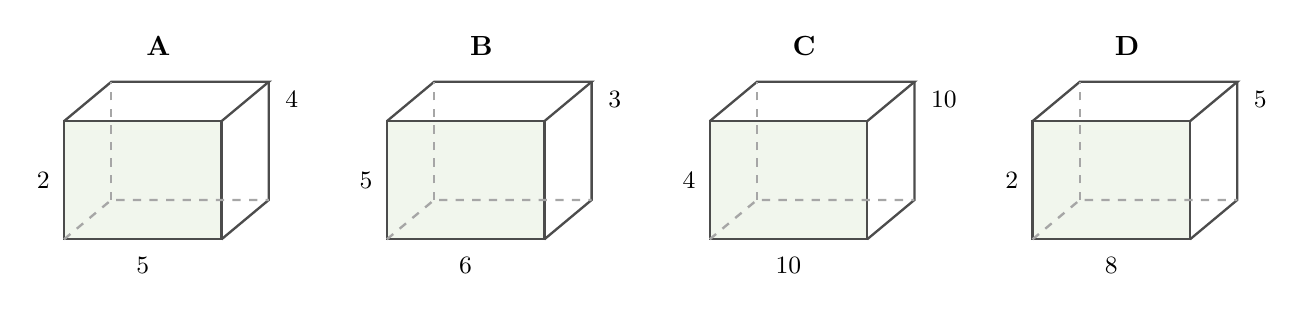
\begin{tikzpicture}[x=1cm, y=1cm, line width=0.85pt, font=\small]

  % Four cuboids in a row. \a/\b/\c are the printed dimensions, not the drawn
  % ones -- every box is drawn the same size on purpose, so the class reads the
  % NUMBERS rather than guessing from the picture.
  \foreach \dx/\lab/\a/\b/\c in {0/A/5/4/2, 4.1/B/6/3/5, 8.2/C/10/10/4, 12.3/D/8/5/2}{
    \begin{scope}[shift={(\dx,0)}]
      \fill[cbgreen!8] (0,0) rectangle (2.0,1.5);
      \draw[black!70] (0,0) rectangle (2.0,1.5);
      \draw[black!70] (0,1.5) -- (0.6,2.0) -- (2.6,2.0) -- (2.0,1.5);
      \draw[black!70] (2.0,0) -- (2.6,0.5) -- (2.6,2.0);
      \draw[black!35, dashed] (0,0) -- (0.6,0.5) -- (2.6,0.5);
      \draw[black!35, dashed] (0.6,0.5) -- (0.6,2.0);
      \node[below, font=\small] at (1.0,-0.1) {\a};
      \node[left,  font=\small] at (-0.05,0.75) {\c};
      % The depth label goes OUTSIDE the top-right slant edge. On the bottom
      % slant it sat on top of the dashed hidden edges and read as if it were
      % labelling the front bottom edge.
      \node[anchor=west, font=\small] at (2.68,1.78) {\b};
      \node[font=\bfseries] at (1.2,2.45) {\lab};
    \end{scope}}

\end{tikzpicture}
\end{center}

\vspace{4pt}
\begin{enumerate}[label=\textbf{\Alph*}, itemsep=13pt, leftmargin=2.2em]
  \item $V \;=\; 5 \times 4 \times 2 \;=\; \mathbf{40\ cm^3}$
  \item $V \;=\; \nbox \times \nbox \times \nbox \;=\; \nbox\ \mathrm{cm^3}$
  \item $V \;=\; \nbox \times \nbox \times \nbox \;=\; \nbox\ \mathrm{cm^3}$
  \item $V \;=\; \nbox \times \nbox \times \nbox \;=\; \nbox\ \mathrm{cm^3}$
\end{enumerate}

% -- E13 --------------------------------------------------------------------
\qhead[cbgreen]{E13}{The tank, one step at a time}

\noindent A tank has a rectangular base measuring $\mathbf{20\ cm}$ by
$\mathbf{10\ cm}$. Mr Bowen pours in water to a depth of $h$ centimetres. Nobody
has measured the depth, so we call it $h$.

\vspace{5pt}
\begin{enumerate}[label=(\alph*), itemsep=13pt]
  \item First, the \textbf{base}. Its area is \;
        $20 \times 10 \;=\; \nbox\ \mathrm{cm^2}$
  \item Now the water. Its volume is the base area \textbf{times} the depth:

        \smallskip
        $V \;=\; \nbox \times h$
  \item Write that the short way, with the number in front of the letter:

        \smallskip
        $V \;=\;$ \blank[3.0cm]
  \item Now use it. When $h = 3$: \hfill
        $V \;=\; \nbox \times 3 \;=\; \nbox\ \mathrm{cm^3}$
  \item And when $h = 7$: \hfill
        $V \;=\; \nbox \times \nbox \;=\; \nbox\ \mathrm{cm^3}$
\end{enumerate}

% -- E14 --------------------------------------------------------------------
% One line of prose between the heading and the box on purpose. Without it the
% heading landed alone at the foot of a page, because a \qhead can fit where the
% tcolorbox after it cannot, and a heading with nothing under it is the worst
% page ending there is.
\qhead[cbgreen]{E14}{Cubic centimetres, millilitres and litres}

\noindent Science measures water in $\mathrm{cm^3}$ and a bottle is labelled in ml.
They are the same thing.

\begin{remember}[Two facts, and that is all]
  $1\ \mathrm{cm^3} = 1\ \mathrm{ml}$ \quad --- exactly the same amount, two names.

  \smallskip
  $1000\ \mathrm{cm^3} = 1\ \mathrm{litre}$
\end{remember}

\vspace{2pt}
\begin{multicols}{2}
\begin{enumerate}[label=(\alph*), itemsep=12pt]
  \item $250\ \mathrm{cm^3} =$ \blank[2.0cm] ml
  \item $2000\ \mathrm{cm^3} =$ \blank[2.0cm] litres
  \item $1500\ \mathrm{cm^3} =$ \blank[2.0cm] litres
  \item $3\ \mathrm{litres} =$ \blank[2.0cm] $\mathrm{cm^3}$
\end{enumerate}
\end{multicols}

\vspace{4pt}
\noindent \textbf{(e)} A water bottle holds $500\ \mathrm{ml}$. A measuring cylinder
in the science lab is marked in $\mathrm{cm^3}$. How many $\mathrm{cm^3}$ of water
does the bottle hold? \hfill \blank[3.4cm]

\vspace{8pt}
\noindent \textbf{(f)} The tank in \textbf{E13} holds $200h\ \mathrm{cm^3}$ of water.
Mr Bowen fills it to a depth of $h = 25\ \mathrm{cm}$. How many \textbf{litres} is
that?
\qlines{3}

% -- E15 --------------------------------------------------------------------
% The last question, and the only one on the sheet that is not arithmetic. It
% is the Section C idea from Homework 6 -- l, w and h all change while lwh does
% not -- reduced to four ticks and a two-word sentence.
\qhead[cbgreen]{E15}{Say what changed}

\noindent Mr Bowen pours the \textbf{same} $200\ \mathrm{cm^3}$ of water from a tall
narrow cylinder into a wide flat dish. Nothing is added and nothing is spilled.

\vspace{7pt}
\noindent Tick one box in each row.

\vspace{6pt}
\noindent
\begin{tabularx}{\textwidth}{|X|c|c|}
  \hline
  & \textbf{Changes} & \textbf{Stays the same} \\
  \hline
  How \textbf{long} the water is \rule[-0.65em]{0pt}{2.0em}   & & \\ \hline
  How \textbf{wide} the water is \rule[-0.65em]{0pt}{2.0em}   & & \\ \hline
  How \textbf{deep} the water is \rule[-0.65em]{0pt}{2.0em}   & & \\ \hline
  The \textbf{volume} of the water \rule[-0.65em]{0pt}{2.0em} & & \\ \hline
\end{tabularx}

\vspace{10pt}
\noindent Now finish the sentence. Use each word \textbf{once}:
\;\eng{shape}\quad\eng{volume}

\vspace{8pt}
\noindent A liquid keeps the same \blank[3.4cm] but takes the \blank[3.4cm] of its
container.

% ===========================================================================
% ANSWER KEY -- TEACHER COPY ONLY
% ===========================================================================
\ifkey
\clearpage

\hwsection[cbred]{Answer Key --- Teacher Copy}

\linespread{1.0}\selectfont
\setlist[enumerate]{itemsep=2pt, topsep=3pt, leftmargin=*}
\setlist[itemize]{itemsep=2pt, topsep=3pt, leftmargin=*}

\qhead[cbred]{E1}{The bag you cannot see into}
\noindent (a) \textbf{2} \quad (b) \textbf{5} \quad (c) \textbf{any letter}, with
$n$, $b$ and $x$ all equally right.

\smallskip
\noindent{\small The answer to (c) is a letter, and \emph{which} letter does not
matter --- say that out loud, because a student who thinks there is a correct letter
to guess has misunderstood the whole idea. What does matter is that they wrote
something. A blank in (c) means the student believes a question with no number has no
answer, and that belief will cost them every mark in Unit 2.}

\qhead[cbred]{E2}{Put three more in}
\noindent (a) $6+3 = \mathbf{9}$ \quad (b) $\mathbf{10} + 3 = \mathbf{13}$ \quad
(c) $\mathbf{n} + 3$ \quad (d) $\mathbf{n} - \mathbf{4}$

\smallskip
\noindent{\small The ladder is the point: (a) is arithmetic, (b) is the same
arithmetic with the first number handed over, and (c) is the same sentence again with
a letter in it. Nothing changed except that we stopped being told the number. \\
Expect (c) to be answered $\mathbf{n3}$ or left blank. Neither is a maths error. The
first is notation and is fixed in E3; the second is the belief that an answer must be
a single number, and it is fixed by saying \emph{you are allowed to stop} as often as
it takes.}

\qhead[cbred]{E3}{Say it the short way}
\noindent (b) $7k$ \quad (c) $mp$ \quad (d) $3ab$ \quad (e) $\dfrac{w}{2}$ \quad
(f) $\dfrac{t}{5}$

\smallskip
\noindent{\small Watch for $k7$ in (b). The number goes in front, always, and it is
worth correcting on sight rather than in writing. \\
Accept $w \div 2$ for (e) and (f) today, but write the fraction beside it --- the
workbook and the exam both use the fraction, and a student who has only ever seen
$\div$ will not recognise it.}

\qhead[cbred]{E4}{One beaker, four things to do to it}
\noindent (a) $b + 40$ \quad (b) $b - 25$ \quad (c) $3b$ \quad
(d) $\dfrac{b}{2}$

\smallskip
\noindent{\small All four answers are unfinished, and all four are correct. This is
the same question the workbook asks about a box of toys, moved into the beaker the
class handled in Science, so the letter has something real behind it. \\
If a student invents a number for $b$ and answers everything in numbers, they have
done four correct calculations and answered none of the questions. Do not mark it
wrong --- ask them what $b$ is, wait, and let them arrive at ``we do not know''.}

\qhead[cbred]{E5}{Match the description to the expression}
\noindent a--\textbf{i} \quad b--\textbf{iv} \quad c--\textbf{v} \quad
d--\textbf{vi} \quad e--\textbf{ii} \quad f--\textbf{iii}. \;
Left over: \textbf{vii} $(8x-8)$.

\smallskip
\noindent{\small \textbf{This is the best question on the sheet.} Every description
uses 3 and 8 and nothing else, so there is no arithmetic anywhere in it --- the only
thing being tested is reading, which is exactly the barrier in this class. \\
The pairs to mark together are \textbf{c and d} ($3x-8$ against $8-3x$) and
\textbf{e and f} ($8x-3$ against $3-8x$). One word, \emph{from}, is the entire
difference. A student who gets c and e right and d and f wrong has read every word
except that one, and that is a very specific, very fixable diagnosis. \\
The left-over expression matters too: a student who forces a match for vii has assumed
every box must be used, which is the same instinct as inventing a number for $b$.}

\qhead[cbred]{E6}{Expression or formula?}
\noindent (c) E \quad (d) F \quad (e) E \quad (f) F \quad (g) E \quad (h) F

\smallskip
\noindent{\small Six items, one rule, thirty seconds. It is here to be got right ---
after E5 the class needs a question it can finish. \\
The only wobble is (h), $P = 2l+2w$, because it is longer than the others. Length is
not the test; the equals sign is.}

\qhead[cbred]{E7}{The same expression, four times}
\noindent (a) $m=2 \to 9$, \; $m=5 \to 12$, \; $m=9 \to 16$. \\
(b) $m=2 \to 8$, \; $m=5 \to 20$, \; $m=9 \to 36$.

\smallskip
\noindent{\small Column (b) is the whole reason the two lists are printed side by
side. In (a) the letter is replaced and the sentence reads the same way; in (b) the
letter is replaced and a hidden times sign has to come back. \\
The errors to expect are \textbf{42}, \textbf{45} and \textbf{49} in column (b) ---
the digits pushed together. A student making that error is not confused about
multiplication; they are reading $4m$ as a two-digit number. Write $4 \times m$ over
the top of it on their page.}

\qhead[cbred]{E8}{The middle line, with the numbers left out}
\begin{enumerate}[label=(\alph*), itemsep=3pt]
  \item $5 \times 7 = \mathbf{35}$
  \item $7 + 12 = \mathbf{19}$
  \item $3 \times 6 + 4 = 18 + 4 = \mathbf{22}$
  \item $20 - 2 \times 8 = 20 - 16 = \mathbf{4}$
  \item $36 \div 4 = \mathbf{9}$
  \item $2 \times 5 + 3 \times 2 = 10 + 6 = \mathbf{16}$
\end{enumerate}
\noindent{\small \textbf{This is the sheet in miniature.} The middle line is printed
with the numbers missing, so it cannot be skipped --- filling the boxes \emph{is} the
method. A student who can fill these in and still writes 34 for $3n$ on the main
packet has not transferred the habit, and the fix is to make them draw the boxes
themselves for a week. \\
(d) is the one that goes wrong. The multiplication is written second and happens
first; a student working strictly left to right gets $18 \times 8 = 144$. The printed
skeleton makes that almost impossible, which is the point --- and is also why the
same question without the skeleton belongs on the next sheet, not this one.}

\qhead[cbred]{E9}{True or false}
\noindent (b) \textbf{True} \quad (c) \textbf{True} \quad
(d) \textbf{False}; $6 \times 3 = \mathbf{18}$ \quad
(e) \textbf{True} \quad (f) \textbf{False}; $4 + 2 \times 5 = 4 + 10 = \mathbf{14}$

\smallskip
\noindent{\small Three of the five are true, deliberately. A sheet where everything is
wrong teaches students to answer \emph{false} without reading. \\
(d) is the digits-pushed-together error again, and it should now be spotted instantly
after E7. \\
(f) is the order-of-operations error, and it is the harder one: 30 comes from doing
$4+2=6$ and then $6 \times 5$. Both numbers in that wrong answer are real numbers from
the question, which is what makes it convincing. Ask the student to write the middle
line from E8 and it collapses on its own.}

\qhead[cbred]{E10}{Two formulae, one rectangle}
\noindent
\begin{tabularx}{\linewidth}{@{}ccXX@{}}
  $l$ & $w$ & $A = lw$ & $P = 2l+2w$ \\
  5   & 3   & $5 \times 3 = 15$   & $10 + 6 = 16$ \\
  8   & 2   & $8 \times 2 = 16$   & $16 + 4 = 20$ \\
  10  & 6   & $10 \times 6 = 60$  & $20 + 12 = 32$ \\
  7   & 7   & $7 \times 7 = 49$   & $14 + 14 = 28$ \\
\end{tabularx}

\smallskip
\noindent{\small The 8-by-2 row is worth pointing at: the area and the perimeter are
16 and 20, two numbers of similar size, and a student who has muddled the two formulae
will not notice from the answer. The 10-by-6 row separates them properly. \\
The 7-by-7 row is a square. Nobody has to be told; it is there so that somebody
notices, and if a student says ``that one is a square'' the lesson has landed.}

\qhead[cbred]{E11}{Count the letters, then write the unit}
\noindent
\begin{tabularx}{\linewidth}{@{}p{3.4cm}Xp{3.0cm}@{}}
  $lwh$                 & three & $\mathrm{cm^3}$ \\
  $3ab$                 & \textbf{two} --- the 3 is not a length & $\mathrm{cm^2}$ \\
  $s \times s \times s$ & three & $\mathrm{cm^3}$ \\
\end{tabularx}

\smallskip
\noindent{\small $3ab$ is the row that teaches something. There are three symbols and
only \emph{two} of them are lengths --- 3 is just a count, so it does not carry a
centimetre. Three rectangles of area $ab$ is still an area. \\
Expect $\mathrm{cm^3}$ for that row from most of the class, and treat it as a
discussion rather than a cross: the rule they extracted, ``count the things being
multiplied'', is a reasonable rule and it is nearly right. The correction is one word:
count the \emph{lengths}.}

\qhead[cbred]{E12}{Find the volume of each box}
\noindent \textbf{A} $= 5 \times 4 \times 2 = \mathbf{40\ cm^3}$ \quad
\textbf{B} $= 6 \times 3 \times 5 = \mathbf{90\ cm^3}$ \\
\textbf{C} $= 10 \times 10 \times 4 = \mathbf{400\ cm^3}$ \quad
\textbf{D} $= 8 \times 5 \times 2 = \mathbf{80\ cm^3}$

\smallskip
\noindent{\small All four boxes are drawn the same size on purpose. The picture
carries no information at all, so the numbers have to be read --- and a student who
answers ``C is the biggest because it looks biggest'' has been caught by a trap that
was set for exactly that. \\
Box C is $400$, not $40$: $10 \times 10$ is where the zeros get dropped. \\
If anyone answers $\mathbf{11}$ for A, they added the three lengths. That is C5.3 on
the main packet, and it is the reason the unit says 3.}

\qhead[cbred]{E13}{The tank, one step at a time}
\noindent (a) $20 \times 10 = \mathbf{200\ cm^2}$ \quad
(b) $V = \mathbf{200} \times h$ \quad
(c) $V = \mathbf{200h}$ \\
(d) $V = 200 \times 3 = \mathbf{600\ cm^3}$ \quad
(e) $V = 200 \times 7 = \mathbf{1400\ cm^3}$

\smallskip
\noindent{\small The base area is worked out \emph{first}, and as a number, before the
letter ever appears. That is the whole design: by the time $h$ arrives there is only
one multiplication left to write, and $200 \times h$ is not frightening. \\
(c) is the only step with no arithmetic in it and it is the one to check --- writing
$200 \times h$ as $200h$ is E3 arriving in a new place, and a student who writes
$h200$ has the maths right and the notation wrong. \\
(d) is where $200h$ with $h=3$ could come out as $\mathbf{2003}$. The printed skeleton
prevents it here. On the main packet, in C2, it does not.}

\qhead[cbred]{E14}{Cubic centimetres, millilitres and litres}
\noindent (a) $\mathbf{250}$ ml \quad (b) $\mathbf{2}$ litres \quad
(c) $\mathbf{1.5}$ litres \quad (d) $\mathbf{3000\ cm^3}$ \\
(e) $\mathbf{500\ cm^3}$ \quad
(f) $200 \times 25 = 5000\ \mathrm{cm^3} = \mathbf{5}$ litres.

\smallskip
\noindent{\small (a) is meant to look like a trick and is not one: the number does not
change, because a cubic centimetre and a millilitre are the same amount of space with
two different names. Some students will not believe it. Show them a
$1\ \mathrm{cm^3}$ cube and a $1\ \mathrm{ml}$ mark on a syringe. \\
(c) is the only answer on the sheet that is not a whole number. \\
(f) uses the formula built in E13, so it is worth the space. A student who gets
5000 and stops has done the maths and not read the word \emph{litres} --- which is, as
always, the actual difficulty.}

\qhead[cbred]{E15}{Say what changed}
\noindent How long --- \textbf{changes} \quad How wide --- \textbf{changes} \quad
How deep --- \textbf{changes} \quad The volume --- \textbf{stays the same}

\smallskip
\noindent A liquid keeps the same \textbf{volume} but takes the \textbf{shape} of its
container.

\smallskip
\noindent{\small \textbf{This is the only question on the sheet with no arithmetic in
it, and it is the one to talk about.} It is the science property from 2.1a and an
algebraic fact at the same time: three measurements all change, and their product does
not. Neither subject could have said that on its own. \\
The row that decides it is the fourth. A student who ticks \emph{changes} for the
volume has not accepted the sentence they wrote underneath, and pouring
$200\ \mathrm{cm^3}$ between a cylinder and a dish at the front of the room settles it
in twenty seconds. \\
Expect \emph{stays the same} for ``how long'' from a few, on the grounds that it is the
same water. Ask them to hold their hands apart to show the water in the cylinder, then
in the dish.}

\fi

\end{document}
